\pagebreak
\section{Steering Test - Steering Gain} \label{app:steeringOrderTest}
\textbf{Name: Group 510}\\
\textbf{Date: 29/11 - 2015}

\subsection{Purpose}
The purpose of the test is to find the relationship between the velocity and steering gain, \si{K_v}.

% find the needed order of the steering model, and the gain related to the speed during the turning of the vehicle, with a PWM signal as an input and the vehicle's heading angle as an output.

\subsection{Setup}
\begin{figure}[H]
  \centering
	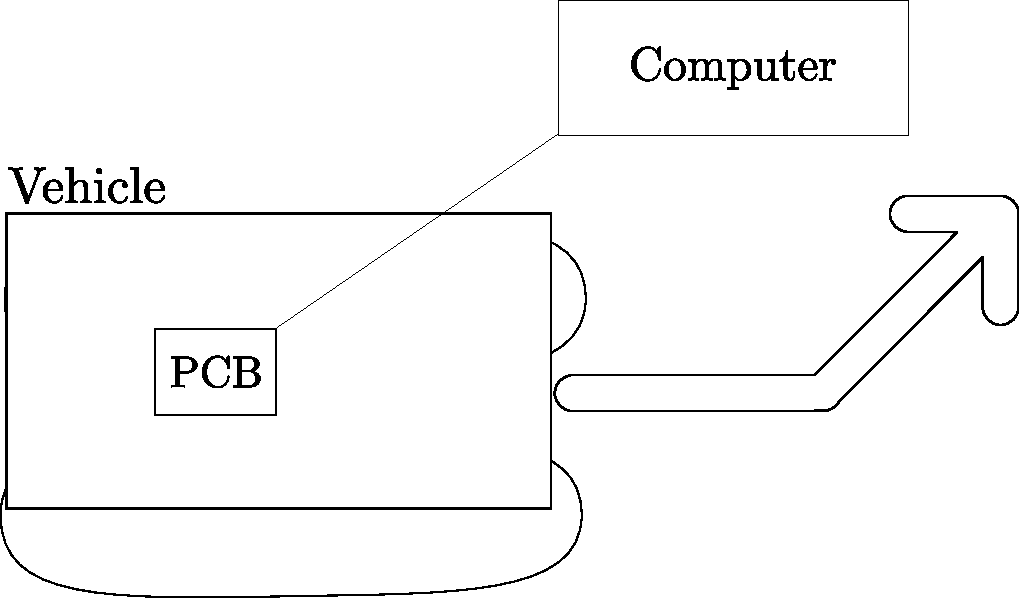
\includegraphics[scale=0.7]{figures/inertiaTestSetupDiagramTurning.pdf}
	\caption{A diagram of the test setup}
\end{figure}

\subsection{List of Equipment}

\begin{table}[H]
\begin{tabular}{|p{10cm}|p{4cm}|}
\hline%------------------------------------------------------------------------------------
  \textbf{Instrument}                     &  \textbf{Type}       \\
\hline%------------------------------------------------------------------------------------
  Computer                                &  Acer C720p    \\
\hline %-----------------------------------------------------------------------------------
\end{tabular}
\end{table}

\subsection{Procedure}

\begin{enumerate}
  \item Disconnect the battery.
  \item Connect the Arduino to the computer.
  \item Upload the test code to the Arduino board using the Arduino IDE  \cite{ArduinoIDE}.
  \item Plug in the battery
  \item Open a serial terminal via PuTTY \cite{PuTTY} immediately after plugging the battery.
  \item Wait two seconds, then follow the vehicle with the connected computer.
  \item Wait until the vehicle stops before ending the measurements by unplugging the connected computer from the Arduino.
  \item Plot the angle of the vehicle using Matlab.
\end{enumerate}

\subsection{Results}

The transfer function of the steering can be expressed as:
\begin{flalign}
\eq{\frac{\theta(s)}{\theta_{ref}(s)}}{\frac{\frac{1}{K_p \cdot K_v}}{1 + \frac{1}{K_p \cdot K_v}}}&
\end{flalign}

And the time constant can be expressed as:
\begin{flalign}
\eq{\tau}{\frac{1}{K_p \cdot K_v}} \unit{s}
\label{SteeringTimeconstant}
\end{flalign}


The different steering time constants can be calculated thanks to the measurements tests. The value of \si{\tau} corresponds to the time when the angle reaches 63,2\% of the final value. A plot of these test can be seen on \figref{plotStepResponseSteering}. 

\begin{figure}[H]
  \centering
 	%Trim margins @:   left        bottom       right       top
 	\adjustbox{ trim = {.15\width} {.30\height} {.15\width} {.30\height}, clip }
  {
    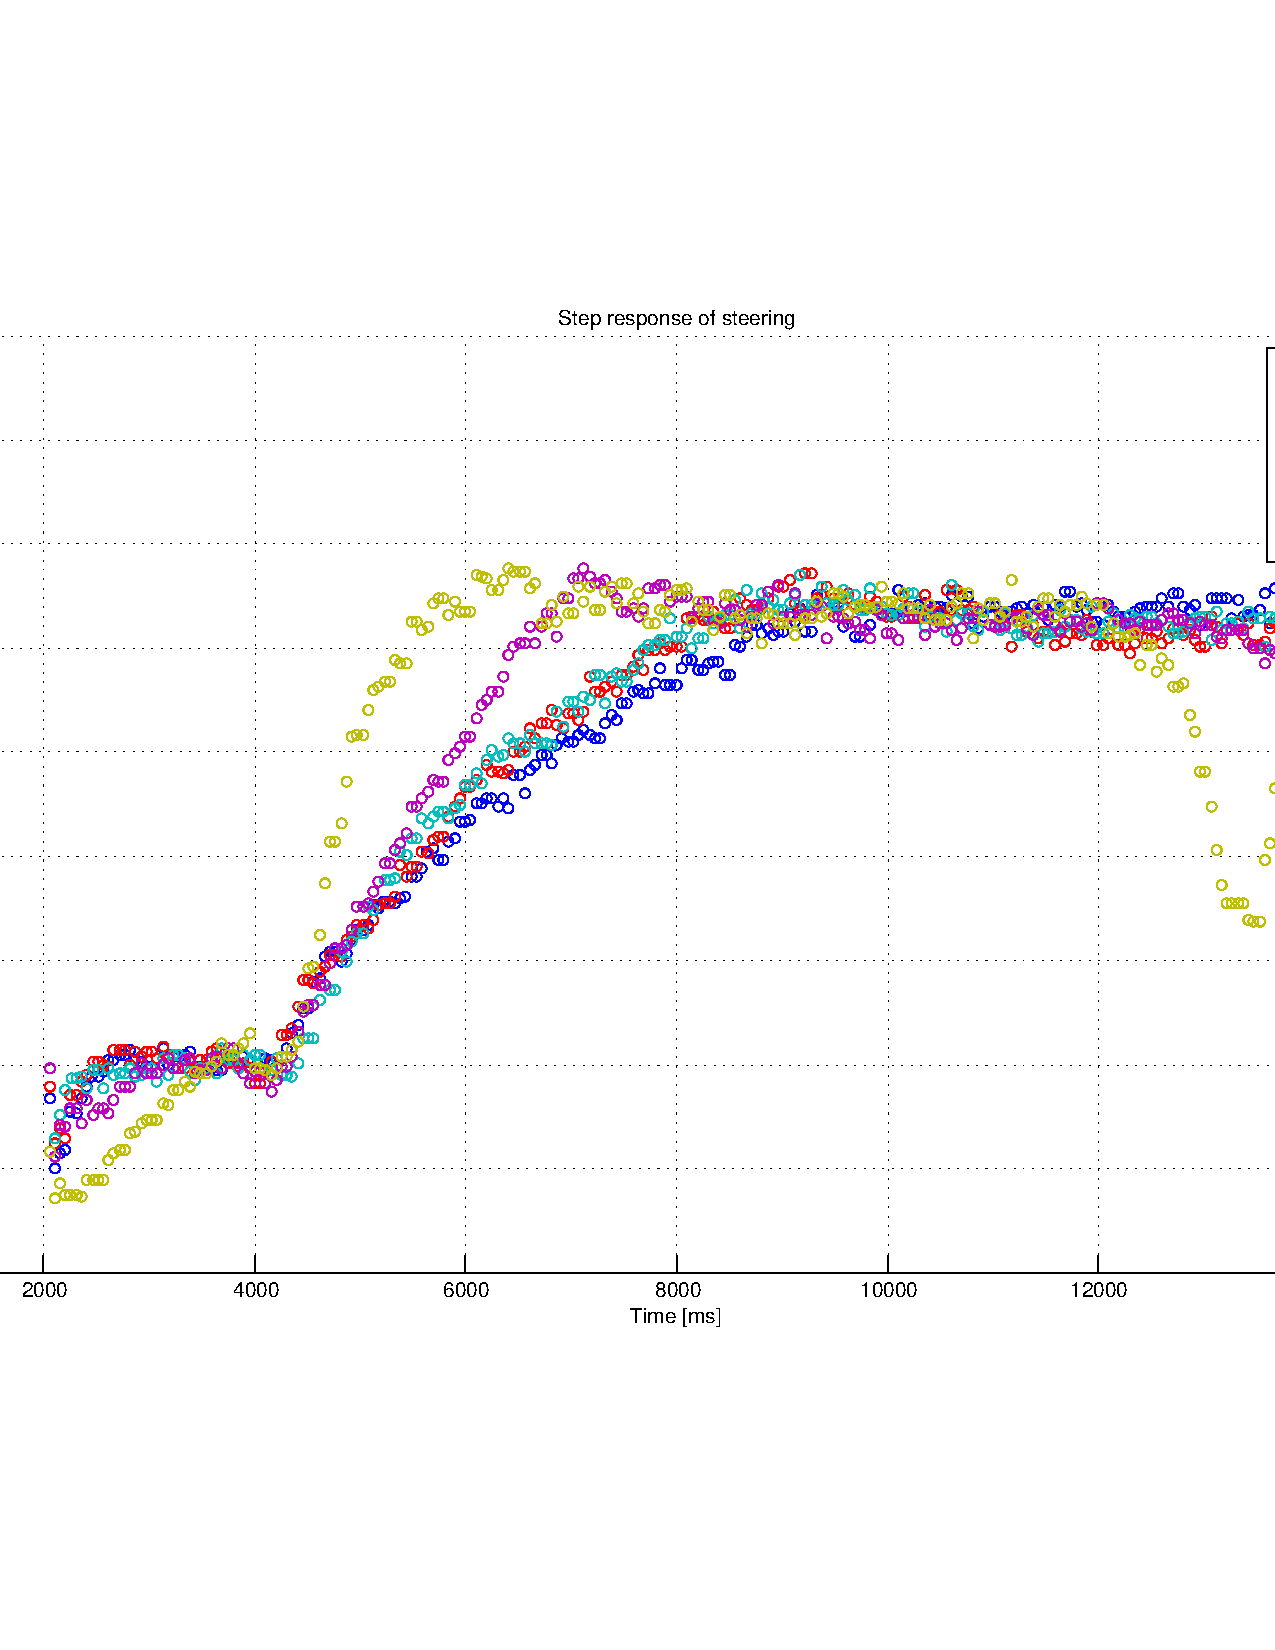
\includegraphics[width=1.4\textwidth]{figures/plotStepResponseSteering.pdf}
  }
  \caption{Plot of multiples step responses for finding the time constant \si{\tau} relative to a specific speed.}
  \label{plotStepResponseSteering}
\end{figure}

As the test were made with a choosen gain K = 1.5, the gain related to the speed during the turning can be calculated:

\begin{flalign}
\eq{K_v}{\frac{1}{K_p \cdot \tau}}
\end{flalign}

A plot of the gain against the speed can be seen on \figref{steeringPlotSpeedVsGain}.

\begin{figure}[H]
  \centering
 	%Trim margins @:   left        bottom       right       top
 	\adjustbox{ trim = {.15\width} {.30\height} {.15\width} {.30\height}, clip }
  {
    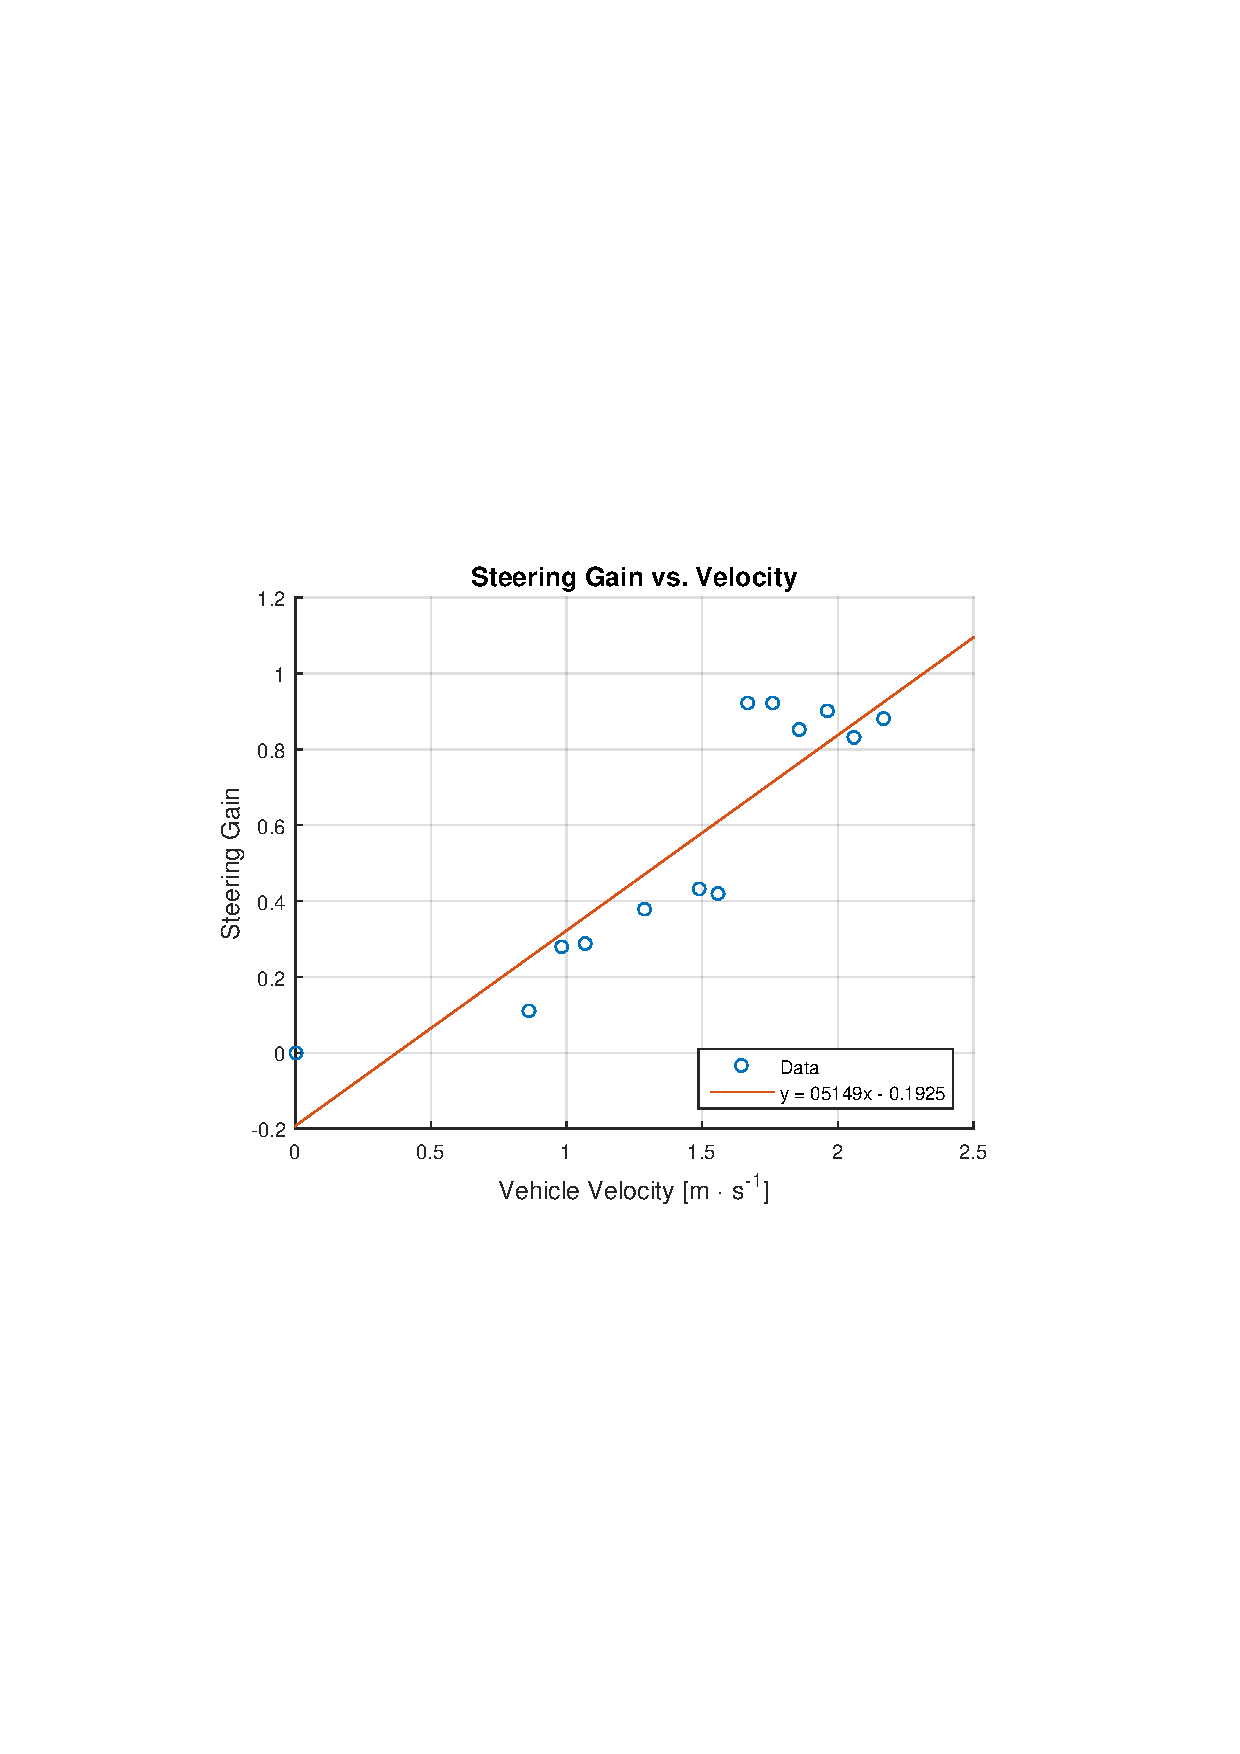
\includegraphics[width=1.4\textwidth]{figures/steeringgainfunction.pdf}
  }
  \caption{Plot of the gain \si{K_v} against the real speed.}
  \label{steeringPlotSpeedVsGain}
\end{figure}

From this plot the linear gain proportional to the speed can be established:
\begin{flalign}
\eq{K_v}{0.5149 \cdot v - 0.1925}
\end{flalign}